\documentclass[submit]{harvardml}

% Put in your full name and email address.
\name{Melissa Yu}
\email{melissayu@college.harvard.edu}

% List any people you worked with.
\collaborators{%
  Alex Lin
}

% You don't need to change these.
\course{CS281-F17}
\assignment{Assignment \#2 v 1.1}
\duedate{5:00pm October 9, 2017}

\usepackage{url, enumitem}
\usepackage{amsfonts}
\usepackage{listings}
\usepackage{bm}

\usepackage{graphicx}
\usepackage{float}
\usepackage{subcaption}
\graphicspath{ {img/} }
\usepackage{epstopdf} % eps to pdf, declare graphics
\DeclareGraphicsRule{.tif}{png}{.png}{`convert #1 `dirname #1`/`basename #1 .tif`.png}

\usepackage{hyperref}
\usepackage{tikz}
\usetikzlibrary{bayesnet}
% Some useful macros.
\newcommand{\given}{\,|\,}
\newcommand{\R}{\mathbb{R}}
\newcommand{\E}{\mathbb{E}}
\newcommand{\var}{\text{var}}
\newcommand{\cov}{\text{cov}}
\newcommand{\N}{\mathcal{N}}
\newcommand{\ep}{\varepsilon}

\newcommand{\Dir}{\text{Dirichlet}}
\newcommand{\Bet}{\text{Beta}}
\newcommand{\Ber}{\text{Bernoulli}}
% Useful macros.
\newcommand{\trans}{\mathsf{T}}
\newcommand{\bx}{\mathbf{x}}
\newcommand{\by}{\mathbf{y}}
\newcommand{\bw}{\mathbf{w}}
\newcommand{\distNorm}{\mathcal{N}}
\newcommand{\bzero}{\mathbf{0}}
\newcommand{\ident}{\mathbb{I}}
\renewcommand{\v}[1]{\mathbf{#1}}

\begin{document}


\noindent \textbf{NOTE:} you must show derivations for your answers unless a question explicitly mentions that no justification is required.

%%%%%%%%%%%%%%%%%%%%%%%%%%%%%%%%%%%%%%%%%%%%%%%%%%%%%%%%
%%%%%%%%%%%%%%%%% PROBLEM 1 %%%%%%%%%%%%%%%%%%%%%%%%%%%%
%%%%%%%%%%%%%%%%%%%%%%%%%%%%%%%%%%%%%%%%%%%%%%%%%%%%%%%%
\begin{problem}[Spherical Gaussian, 10pts]
One intuitive way to summarize a probability density is via the mode,
as this is the ``most likely'' value in some sense.  A common example
of this is using the maximum \textit{a posteriori} (MAP) estimate of a
model's parameters.  In high dimensions, however, the mode becomes
less and less representative of typical samples.  Consider variates
from a~$D$-dimensional zero mean spherical Gaussian with unit
variance:
\begin{align*}
  \bx &\sim \distNorm(\bzero_D, \ident_D),
\end{align*}
where~$\bzero_D$ indicates a column vector of~$D$ zeros and~$\ident_D$
is a~${D\times D}$ identity matrix.
\begin{enumerate}
  \item Compute the distribution that this implies over the distance
    of these points from the origin.  That is, compute the
    distribution over~$\sqrt{\bx^\trans\bx}$, if~$\bx$ is a
    realization from~$\distNorm(\bzero_D, \ident_D)$.  (Note: Consider
    transformations of a Gamma distribution described in Murphy 2.4.5.)
  \item Make a plot that shows this probability density function for
    several different values of~$D$, up to ~${D=100}$.

  \item Make a plot of the cumulative distribution function (CDF) over
    this distance distribution for~${D=100}$.  A closed-form solution
    may be difficult to compute, so you can do this numerically.)

  \item From examining the CDF we can think about where most of the
    mass lives as a function of radius.  For example, most of the mass
    for~${D=100}$ is within a thin spherical shell.  From eyeballing
    the plot, what are the inner and outer radii for the shell that
    contains 90\% of the mass in this case?
\end{enumerate}
\end{problem}


\begin{enumerate}
	\item We have $\bx = \langle x_1, \dots, x_D \rangle$, where the $x_i$ are i.i.d. and distributed $\distNorm(0, 1)$ by the properties of MVN's. We wish to find the distribution of
	\[Y = \sqrt{\bx^\trans\bx} = \sqrt{\sum_{i=1}^D x_i^2}\]
	As described in Murphy 2.4.4, the sum of squared standard normals $S = \sum_{i=1}^D x_i^2$ follows the chi-squared distribution $\chi_D^2$. Taking the square root with the change of variables formula, $\sqrt{S}$ has the pdf
	\[
	f_Y(y) 
	= 2y f_S(y^2)
	= 2y\frac{y^{D-2}e^{-y^2 / 2}}{2^{D/2}\Gamma(D/2)}
	= \frac{2^{1 - D/2} y^{D-1} e^{-y^2/2}}{\Gamma(D/2)},
	\]
	which is the chi distribution with $D$ degrees of freedom.
	
	\item See figure ~\ref{1-2}.
	\begin{figure}
		\centering
		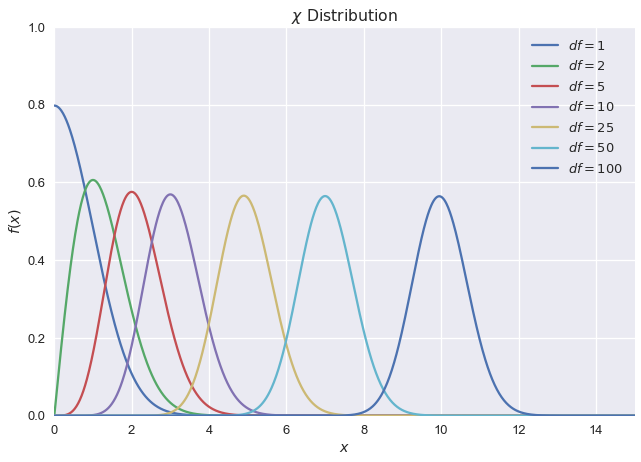
\includegraphics[width=.75\textwidth]{1-2}
		\caption{$\chi$ PDF for various df's.}
		\label{1-2}
	\end{figure}
	
	\item See figure ~\ref{1-3}.
	\begin{figure}
		\centering
		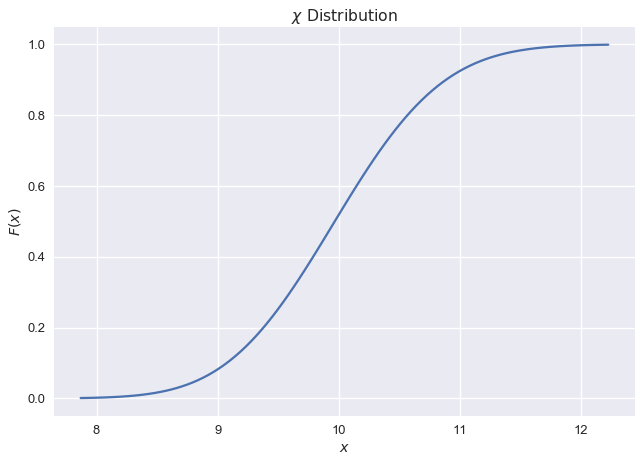
\includegraphics[width=.75\textwidth]{1-3}
		\caption{$\chi$ CDF for 100 degrees of freedom.}
		\label{1-3}
	\end{figure}
	
	\item From examining the CDF, we see that 90\% of the mass lies between $r=9$ and $r=12$, and 80\% between $r=9$ and $r=11$.
\end{enumerate}
\newpage

%%%%%%%%%%%%%%%%%%%%%%%%%%%%%%%%%%%%%%%%%%%%%%%%%%%%%%%%
%%%%%%%%%%%%%%%%% PROBLEM 2 %%%%%%%%%%%%%%%%%%%%%%%%%%%%
%%%%%%%%%%%%%%%%%%%%%%%%%%%%%%%%%%%%%%%%%%%%%%%%%%%%%%%%
\begin{problem}[Hurdle Models for Count Data, 10pts]

  In this problem we consider predictive models of count data. For
  instance given information about the student $x$, can we predict how
  often they went to the gym that week $y$? A natural choice is to use a Poisson GLM
  i.e. $y$ conditioned on $x$ is modeled as a Poisson distribution.

  However, in practice, it is common for count data of this form to
  follow a bi-modal distribution over count data. For instance, our
  data may come from a survey asking students how often they went to
  the gym in the past week. Some would do so frequently, some would do
  it occasionally but not in the past week (a random zero), and a
  substantial percentage would never do so.

  When modeling this count data with generalized linear models, we
  may observe more zero examples than expected from our model.
  In the case of a Poisson, the mode of the distribution is the
  integer part of the mean. A Poisson GLM may therefore be inadequate
  when means can be relatively large but the mode of the output is 0. Such data is
  common when many data entries have 0 outputs and many also have much
  larger outputs, so the mode of output is 0 but the overall mean is
  not near 0. This problem is known as \textit{zero-inflation}.

  This problem considers handling zero-inflation with a two-part model called
  a \textit{hurdle model}. One part is a binary model such as a logistic model
  for whether the output is zero or positive. Conditional on a positive output,
  the ``hurdle is crossed'' and the second part uses a truncated model that
  modifies an ordinary distribution by conditioning on a positive
  output. This model can handle both zero inflation and zero
  deflation.

  Suppose that the first part of the process is governed by
  probabilities $p(y > 0\ |\ x) = \pi $ and $p(y = 0\ | \ x) = 1 - \pi$; and the second part
  depends on  $\{y\in \mathbb{Z} \ |\ y > 0\}$ and follows a probability mass
  function $f(y\ |\ \mathbf{x})$ that is truncated-at-zero. The
  complete distribution is therefore:
\begin{align*}
P(y = 0\ |\ x) & = 1- \pi\\
P(y = j\ |\ x) & = \pi \frac{f(j\ |\ \mathbf{x})}{1 - f(0\ | \ \mathbf{x})},\ j=1,2,...
\end{align*}
One choice of parameterization is to use a logistic regression model
for $\pi$: $$\pi = \sigma(\mathbf{x}^\top \mathbf{w}_1)$$ and use a Poisson GLM for $f$ with mean parameters $\lambda$ (see
Murphy 9.3): $$\lambda = \exp(\mathbf{x}^\top \mathbf{w}_2) $$

\begin{enumerate}[label=(\alph*)]
\item Suppose we observe $N$ data samples $\{(x_n, y_n)\}_{n=1}^N$.  Write down the log-likelihood for the hurdle model assuming an unspecified mass function $f$.
Give an maximum likelihood estimation approach for the specified parts of the model.

\item Assume now that we select Poisson distribution for $f$. Show
  that the truncated-at-zero Poisson distribution (as used in the
  hurdle model) is a member of the exponential family.  Give its the
  sufficient statistics, natural parameters and log-partition
  function.

\item What is the mean and variance of a truncated Poisson model with mean parameter $\lambda$? If we observe $n$ i.i.d. samples from a truncated Poisson distribution, what is the maximum likelihood estimate of $\lambda$? (Note: Give an equation which could be solved numerically to obtain the MLE. )

\item  Now assume that we using a hurdle model as a GLM with $f$ as a Poisson distribution. Show that
  this is a valid GLM (exponential family for $y$), derive its log-likelihood, and give its sufficient statistics.

\end{enumerate}
\end{problem}

\newpage
\begin{enumerate}[label=(\alph*)]
	\item Let $g(y) = \ident(y \neq 0)$ be the binary indicator of the response $y$ being non-zero, and let $h(y, x)$ be the PDF of the truncated-at-zero distribution, where
	\[
	h(y, x) = \frac{f(y\ |\ \mathbf{x})}{1 - f(0\ | \ \mathbf{x})}
	\]
	Then, the log-likelihood of one example is:
	\begin{align*}
	\log p(y_i\given x_i, \bw_1) 
	&= \log \left[ 
	(1 - \pi_i)^{1-g(y_i)} \left(\pi_i h(y_i, x_i)\right)^{g(y_i)}
	\right] \\
	&= (1-g(y_i)) \log (1 - \pi_i) + g(y_i) \left(\log\pi_i + \log h(y_i, x_i)\right) \\
	&= 
	\bigg[
	(1-g(y_i)) \log (1 - \pi_i) + g(y_i) \log\pi_i
	\bigg] + 
	g(y_i) \log h(y_i, x_i)
	\end{align*}
	We have the following total log-likelihood:
	\begin{align*}
	\log p(\mathcal{D}\given\theta)
	&= \sum_{i=1}^N \log p(y_i\given x_i, \bw_1) \\
	&= \left[ \sum_{i=1}^N 
	(1-g(y_i)) \log (1 - \pi_i) + g(y_i) \log\pi_i
	\right] + \left[ \sum_{i=1}^N
	g(y_i) \log h(y_i, x_i)
	\right] \\
	&= \left[ \sum_{i=1}^N 
	(1-g(y_i)) \log (1 - \sigma(\mathbf{x}_i^\top \mathbf{w}_1)) + g(y_i) \log (\sigma(\mathbf{x}_i^\top \mathbf{w}_1))
	\right] + \left[ \sum_{i=1}^N
	g(y_i) (\log f(y_i\ |\ \mathbf{x}_i) + const)
	\right] \\
	&= \ell_1(\bw_1\given\mathcal{D}) + \ell_2(f\given\mathcal{D})
	\end{align*}
	We see that the log-likelihood breaks into two terms, and thus the parameters for $\pi$ and $f$ can be optimized separately. The first term is simply the log-likelihood for a logistic regression model, and we can use second-order optimization methods like IRLS to find $\bw_1$. Similarly, we can calculate the Hessian of $\log f(y_i\ |\ \mathbf{x}_i)$ and estimate the MLE parameters of $f$ using second-order methods.
	
	\item We have $f(y\ |\ \mathbf{x}) = Po(y\given\lambda)$. Rewriting the pdf for the truncated Poisson, we have
	\begin{align*}
	g(y) &= \frac{f(y\ |\ \mathbf{x})}{1 - f(0\ | \ \mathbf{x})} \\
	&= \frac{\lambda^y}{y! (e^{\lambda} - 1)} \\
	&= \frac{1}{y!} \exp\{
	y\log\lambda - \log(e^{\lambda} - 1)
	\} \\
	&= h(y)\exp\{\theta \phi(y) - A(\theta)\},
	\end{align*}
	where $h(y) = \frac{1}{y!}$, $\theta = \log\lambda$, $\phi(y) = y$, and $A(\theta) = \log(e^{e^\theta} - 1)$.
	
	\item Using the results derived in Murphy 9.2.3, we use the log partition function of the truncated Poisson to derive the first and second cumulants of the sufficient statistics (in this case, the variable itself):
	\begin{align*}
	\E(y) &= \E(\phi(y)) = \frac{dA}{d\theta} 
	= \frac{e^{e^\theta} e^\theta}{e^{e^\theta} - 1} = \frac{\lambda e^{\lambda}}{e^{\lambda} - 1}
	\\
	\var(y) &= \var(\phi(y)) = \frac{d^2A}{d\theta^2} \\
	&= \left(\frac{d}{d\lambda} \frac{\lambda e^{\lambda}}{e^{\lambda} - 1}\right) \frac{d\lambda}{d\theta} \\
	&= \left(
	-\frac{\lambda e^{2\lambda}}{(e^{\lambda} - 1)^2}
	+ \frac{\lambda e^{\lambda} + e^{\lambda}}{e^{\lambda} - 1}
	\right) \lambda \\
	&=
	\frac{\lambda^2 + \lambda}{1 - e^{-\lambda}}
	- \frac{\lambda^2}{(1 - e^{-\lambda})^2}
	\end{align*}
	The log-likelihood of $n$ samples $\mathcal{D} = \{y_i\}_{i=1}^n$ is
	\begin{align*}
	\log p(\mathcal{D}\given\theta) 
	&= \log\left(
	\left[\prod_{i=1}^{n} h(y_i)\right]
	\exp\{\theta\sum_{i=1}^n\phi(y_i) - nA(\theta)\} 
	\right) \\
	&= \sum_{i=1}^{n} \log h(y_i)
	+ \theta\sum_{i=1}^n\phi(y_i) 
	- nA(\theta) \\
	&= \theta\sum_{i=1}^n\phi(y_i) - nA(\theta) + const
	\end{align*}
	Taking the derivative w.r.t. $\theta$, we obtain 
	\begin{align*}
	\frac{d}{d\theta} \log p(\mathcal{D}\given\theta) 
	= \sum_{i=1}^n\phi(y_i) - nA'(\theta)
	= \sum_{i=1}^n\phi(y_i) - n\E(\phi(y))
	\end{align*}
	Thus, at the MLE estimate $\hat{\theta}$, 
	\[
	\E(\phi(y)) = \frac{1}{n} \sum_{i=1}^n\phi(y_i)
	\]
	Substituting in the problem's specifications, we have the following relation for the MLE estimate for $\hat{\lambda}$:
	\begin{align*}
	\frac{\hat{\lambda} e^{\hat{\lambda}}}{e^{\hat{\lambda}} - 1}
	= \frac{1}{n} \sum_{i=1}^n y_i
	\end{align*}
	
	\item Let $\tilde{y} = \ident(y \neq 0)$. We write the pdf of the hurdle model as
	\begin{align*}
	f(y) 
	&= (1 - \pi)^{1-\tilde{y}} \left(\pi \frac{\lambda^y}{y! (e^{\lambda} - 1)}\right)^{\tilde{y}} \\
	&= \frac{1}{y!} \exp\bigg\{
	y\log\lambda + \tilde{y} \log\frac{\pi}{(1 - \pi)(e^{\lambda} - 1)}
	+ \log (1 - \pi) \bigg\} \\
	&= h(y) \exp\{\bm{\theta}^\trans\bm{\phi}(y) - A(\bm{\theta})\},
	\end{align*}
	where
	\begin{align*}
	\bm{\theta} &= \left[\log\lambda, \ \log\frac{\pi}{(1 - \pi)(e^{\lambda} - 1)}\right] \\
	\bm{\phi}(y) &= \big[y, \ \ident(y\neq 0)\big] \\
	A(\bm{\theta}) &= \log(1 - \pi)
	\end{align*}
	
	Using the general results derived earlier in (c), the log-likelihood for the hurdle model is:
	\begin{align*}
	\log p(\mathcal{D}\given\bm{\theta}) &= \bm{\theta}^\trans\sum_{i=1}^n\bm{\phi}(y_i) - nA(\bm{\theta}) + const \\
	&= 
	\log\lambda \left[\sum_{i=1}^n y_i\right]
	+ \log\frac{\pi}{(1 - \pi)(e^{\lambda} - 1)} \left[\sum_{i=1}^n \ident(y_i \neq 0)\right]
	- n\log(1 - \pi) + const,
	\end{align*}
	and the sufficient statistics are $n$ and
	\[
	\bm{\phi}(\mathcal{D}) = \left[
	\sum_{i=1}^n y_i, \
	\sum_{i=1}^n \ident(y_i \neq 0)
	\right]
	\]
\end{enumerate}

%%%%%%%%%%%%%%%%%%%%%%%%%%%%%%%%%%%%%%%%%%%%%%%%%%%%%%%%
%%%%%%%%%%%%%%%%% PROBLEM 3  %%%%%%%%%%%%%%%%%%%%%%%%%%%
%%%%%%%%%%%%%%%%%%%%%%%%%%%%%%%%%%%%%%%%%%%%%%%%%%%%%%%%

\begin{problem}[Directed Graphical and  Naive Bayes, 10pts]
\textit{To draw the DGMs for this problem, we recommend using the \texttt{tikzbayesnet} library. For example the following is drawn in \LaTeX:}
\begin{center}


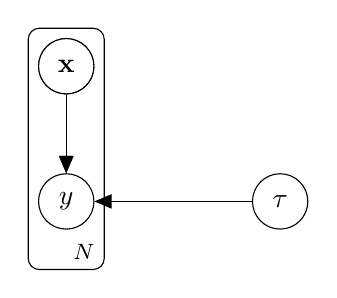
\begin{tikzpicture}
  %Define nodes
  \node[latent]                               (y) {$y$};
  \node[latent, above=of y] (w) {$\mathbf{w}$};
  \node[latent, above=of y]  (x) {$\mathbf{x}$};
  \node[latent, right=2cm of y]            (t) {$\tau$};

  % Connect the nodes
  \edge {x,w,t} {y} ; %

  % Plates
  \plate {yx} {(x)(y)} {$N$} ;

\end{tikzpicture}
\end{center}


\noindent  This problem focuses on modeling a joint distribution of random variables,
$p(y, x_1, \ldots, x_V)$, consisting of discrete variables. These variables represent a class label $y
\in \{1, \ldots, C\}$ and features $x_1 \ldots, x_V$
each of each can take on a values $x_{v} \in \{0, 1\}$.


\begin{enumerate}[label=(\alph*)]
\item  Let $V = 4$. Use the chain rule to select any valid factorization of this joint distribution into univariate distributions. Draw the directed graphical model corresponding to this factorization.

\item What is the sum of the sizes of the \textit{conditional probability tables} associated with
this graphical model. Can you reduce the order of magnitude of this value with a different DGM?

\item  Now consider a naive Bayes factorization of this model, given by,

\[ p(y, x_1, \ldots, x_V ) \approx p(y) \prod_{v} p(x_v | y). \]

Draw a directed graphical model for this factorization.
What is the size of the conditional probability tables required to
fully express any factored distribution of this form?

\item In class, we parameterized naive Bayes such that the class
  distribution is Categorical with a Dirichlet prior, and the
  class-conditional distributions are Bernoulli with a Beta
  prior. Extend the graphical model above to show the generative model
  of $N$ data points and include the parameters and hyper-parameters
  as random variables.


\item Assuming the data obeys the naive Bayes assumptions, answer the following questions as true/false using your directed graphical model.  Justify your answer.

      \begin{itemize}
      \item For a given example, features $x_1$ and $x_2$ are independent.
      \item The class labels $y$ are always conditionally independent of the class-conditional parameters.
      \item Upon observing the class distribution parameters, the class labels are conditionally independent.
      \item Upon observing the class distribution parameters, the features are conditionally independent.
      \item Upon observing the class distribution hyper-parameters, the class labels are conditionally independent.
      \end{itemize}


    \item For the next problem, we will utilize naive Bayes for a
      problem where each example has a \textit{bag} or multiset of
      items. A bag is a set that may contain multiple instances of the
      same value. One approach is to ignore this property and use
      $x_v$ as an indicator function for each item type. An
      alternative is to model $x_v$ with sample space
      $\{0,\ldots, D\}$, where $D$ is the maximum times an item
      appears and to use a Dirichlet-Categorical for the
      class-conditional.  Give one benefit and one drawback of this
      approach. Propose a third option for modeling this distribution.

\end{enumerate}
\end{problem}

\begin{enumerate}[label=(\alph*)]
	\item We choose the factorization
	\[
	p(y, x_{1:4}) = 
	p(x_1) 
	p(x_2\given x_1) 
	p(x_3\given x_{1:2}) 
	p(x_4\given x_{1:3}) 
	p(y\given x_{1:4}),
	\]
	where the MATLAB-like notation $x_{1:V}$ denotes $x_1,\dots,x_V$. The DGM is shown below.
	\begin{center}
		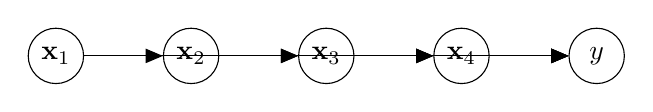
\begin{tikzpicture}
		\node[latent] (x1) {$\mathbf{x}_1$};
		\node[latent, right=of x1] (x2) {$\mathbf{x}_2$};
		\node[latent, right=of x2] (x3) {$\mathbf{x}_3$};
		\node[latent, right=of x3] (x4) {$\mathbf{x}_4$};
		\node[latent, right=of x4] (y)  {$y$};
		
		\edge {x1} {x2} ;
		
		\edge [bend left] {x1} {x3} ;
		\edge {x2} {x3} ;
		
		\edge [bend left] {x1} {x4} ;
		\edge [bend left] {x2} {x4} ;
		\edge {x3} {x4} ;
		
		\edge [bend right] {x1} {y} ;
		\edge [bend right] {x2} {y} ;
		\edge [bend right] {x3} {y} ;
		\edge {x4} {y} ;	
		\end{tikzpicture}
	\end{center}

	\item The sum of the sizes of the CPT's for the DGM factored as in (a) with $V$ binary variables $x_i$ is
	\[
	C2^V + \sum_{i=1}^V 2^i = C2^V + 2^{V+1} - 1
	\]
	Thus, for $V=4$, we have a total CPT size of $16C + 31$. Note that all possible factorizations of the joint result in CPT's with size $O(C2^V)$, since the only difference in the factorizations is at what point $y$ is added to the chain rule. 
	
	\item The size of the CPT's for this factorization is
	\[
	C + \sum_{i=1}^V 2C = C(1 + 2V)
	\]
	The DGM is shown below.
	\begin{center}
		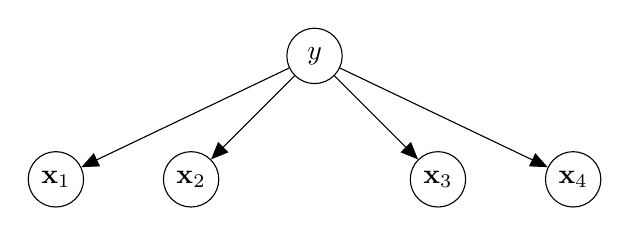
\begin{tikzpicture}
		\node[latent] (y)  {$y$};
		\node[latent, below left=1.5cm of y] (x2) {$\mathbf{x}_2$};
		\node[latent, left=of x2] (x1) {$\mathbf{x}_1$};
		\node[latent, below right=1.5cm of y] (x3) {$\mathbf{x}_3$};
		\node[latent, right=of x3] (x4) {$\mathbf{x}_4$};

		\edge {y} {x1,x2,x3,x4} ;	
		\end{tikzpicture}
	\end{center}
	
	\item The DGM is shown below.
	\begin{center}
		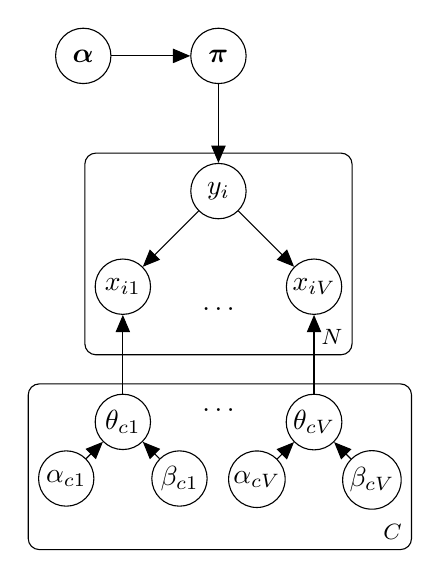
\begin{tikzpicture}
		\node[latent] (pi) 				{$\bm{\pi}$} ;
		\node[latent, left=of pi] (a) 	{$\bm{\alpha}$} ;
		\node[latent, below=of pi] (y) 	{$y_i$} ;
		
		\node[latent, below left=of y]  (x1)	{$x_{i1}$} ;
		\node[latent, below right=of y] (xV)	{$x_{iV}$} ;
		
		\node[latent, below=of x1] (p1) 	{$\theta_{c1}$} ;
		\node[latent, below=of xV] (pV) 	{$\theta_{cV}$} ;
		
		\node[latent, below left=0.3cm of p1] (b1l) 	{$\alpha_{c1}$} ;
		\node[latent, below right=0.3cm of p1] (b1r) 	{$\beta_{c1}$} ;
		
		\node[latent, below left=0.3cm of pV] (bVl) 	{$\alpha_{cV}$} ;
		\node[latent, below right=0.3cm of pV] (bVr) 	{$\beta_{cV}$} ;
		
		\node[below=of y] (dots1) {$\dots$} ;
		\node[below=of dots1] (dots2) {$\dots$} ;

		\edge {a} 	{pi} ;
		\edge {pi} 	{y} ;
		\edge {y} 	{x1, xV} ;
		\edge {p1} 	{x1} ;
		\edge {pV} 	{xV} ;
		\edge {b1l, b1r} 	{p1} ;
		\edge {bVl, bVr} 	{pV} ;
		
		\plate {} {(y)(x1)(xV)} {$N$} ;
		\plate {} {(p1)(pV)(b1l)(b1r)(bVl)(bVr)} {$C$} ;
		\end{tikzpicture}
	\end{center}
	
	\item 
	\begin{itemize}
		\item False. For a given example, features $x_1$ and $x_2$ are conditionally independent, given the class $y$. If $y$ is in the evidence, then features $x_1$ and $x_2$ are d-separated. 
		\item False. The class labels $y$ are not always conditionally independent of the class-conditional parameters. E.g., given the class distribution parameter $\bm{\pi}$, the node $y_i$ and the node $\theta_{c1}$ are not d-separated.
		\item True. Upon observing the class distribution parameters, the class labels are conditionally independent. Each $y_i$ is d-separated by $\bm{\pi}$, which blocks all paths between nodes.
		\item False. Upon observing the class distribution parameters, the features are not d-separated, since $y_i$ is not a blocking node.
		\item False. Upon observing the class distribution hyper-parameters, the class labels are not d-separated by any evidence nodes, since $\bm{\pi}$ is unobserved.
	\end{itemize}

	\item The bag-of-words model is simple and memory-efficient way to represent a text as a histogram over words. However, this representation throws away the syntax and ordering of the words, e.g. so that the phrases ``toy poodle'' and ``poodle toy'' are equivalent. An alternative way to model the distribution is to use the tf-idf statistic instead of the raw count of word $i$. The tf-idf statistic grows proportionally with the count of the word in the document, but scales inversely with the fraction of the documents that contain the word, so that words that are common across the corpus are assigned low values, while terms ``unique'' to a document are given greater weight.
\end{enumerate}

%%%%%%%%%%%%%%%%%%%%%%%%%%%%%%%%%%%%%%%%%%%%%%%%%%%%%%%%
%%%%%%%%%%%%%%%%% PROBLEM 4 %%%%%%%%%%%%%%%%%%%%%%%%%%%%
%%%%%%%%%%%%%%%%%%%%%%%%%%%%%%%%%%%%%%%%%%%%%%%%%%%%%%%%
\begin{problem}[Naive Bayes Implementation, 10pts]

\noindent You will now implement a naive Bayes classifier for
for sentiment classification. For this problem you will use
the IMDB Movie Reviews dataset which consists of positive and negative movie reviews . Here are two example reviews:\\

        \texttt{there is no story! the plot is hopeless! a filmed based on a car with a \\
        \indent stuck accelerator, no brakes, and a stuck automatic transmission gear \\
        \indent lever cannot be good! ...  i feel sorry for the actors ... poor script ... \\
        \indent heavily over-dramatized ... this film was nothing but annoying, \\
        \indent stay away from it!} [negative review] \\

        \texttt{i had forgotten both how imaginative the images were, and how witty \\
        \indent the movie ... anyone interested in politics or history will love the movie's \\
        \indent offhand references - anyone interested in romance will be moved - this \\
        \indent one is superb.} [positive review] \\

      \noindent As noted in the last problem, it is common to think of
      the input data as a bag/multiset. In text applications,
      sentences are often represented as a \textit{bag-of-words},
      containing how many times each word appears in the sentence. For
      example, consider two sentences:
\begin{itemize}
\item \begin{verbatim}We like programming. We like food.\end{verbatim}
\item \begin{verbatim}We like CS281.\end{verbatim}
\end{itemize}
A vocabulary is constructed based on these two sentences:
\begin{verbatim}
                 ["We", "like", "programming", "food", "CS281"]
\end{verbatim}
Then the two sentences are represented as the number of occurrences of each word in the vocabulary (starting from position 1):
\begin{itemize}
\item \begin{verbatim}[0, 2, 2, 1, 1, 0]\end{verbatim}
\item \begin{verbatim}[0, 1, 1, 0, 0, 1]\end{verbatim}
\end{itemize}

\noindent We have included a utility file \texttt{utils.py} that does this mapping. For
these problems you can therefore treat text in this matrix representation.


\begin{itemize}

	\item Implement a Naive Bayes classifier using a
          Bernoulli class-conditional with a Beta prior
          where each feature is an indicator that
          a word appears at least once in the bag.

    \item Implement a Naive Bayes classifier using a Categorical
          class-conditional with a Dirichlet prior. Here
          the features represent that count of each word in
          the bag.



    \item For both models, experiment with various settings
          for the priors. For the Dirichlet prior on
          the class, begin with $\boldsymbol{\alpha} = \v 1$
          (Laplace Smoothing).
          Do the same for the class-conditional prior
          (be it Dirichlet or Beta). Keeping uniformity,
          vary the magnitude to $.5$ and smaller. If the
          classes are unbalanced in the dataset, does it help
          to use a larger $\alpha$ for the less-often occuring
          class? Optionally, choose class-conditional priors based on an
          outside text source. Validate your choices on the validation set,
          and report accuracy on the test set.

      \item (Optional) With the bag-of-words representation, 
             would the model be able to capture phrases
             like ``don't like''? An alternative to the bag-of-words model is
          known as the bag-of-bigrams model, where a bigram is two
          consecutive words in a sentence.  Modify \texttt{utils.py}
          to include bigram features with either model and see if they
          increase accuracy.

    \item (Optional Reading) \textit{Baselines and Bigrams: Simple, Good Sentiment and Topic Classification}\\
    \url{http://www.aclweb.org/anthology/P/P12/P12-2.pdf#page=118}\\
\end{itemize}
\end{problem}


See jupyter notebook for code. For $\bm{\alpha} = 1$, $\bm{\beta} = 1$ we obtain a test accuracy of 86.2\%. Here, we have perfectly balanced class counts, so all uniform values for $\bm{\alpha}$ will yield the same results. Thus, we only vary $\bm{\beta}$ in our tests. The validation accuracies for various values are shown in the table below; we can see that larger pseudo-counts result in higher testing accuracy, but that the difference is fairly small. 

\begin{center}
\begin{tabular}{c|c|c|c}
	$\beta$ & 0.1 & 0.5 & 1 \\ \hline
	acc	(binary feats.)	& 84.2 & 85.6 & 86.1 \\
	acc	(categorical feats.) & 84.4 & 85.9 & 86.2
\end{tabular}
\end{center}

When the classes in a dataset are imbalanced, the weights will be lower for the class with less training data, and classification will thus be incorrectly biased towards one class over the other. Using a non-uniform prior $\bm{\alpha}$ can substantially improve classification performance.

\newpage
%%%%%%%%%%%%%%%%%%%%%%%%%%%%%%%%%%%%%%%%%%%%%%%%%%%%%%%%
%%%%%%%%%%%%%%%%% PROBLEM 5 %%%%%%%%%%%%%%%%%%%%%%%%%%%%
%%%%%%%%%%%%%%%%%%%%%%%%%%%%%%%%%%%%%%%%%%%%%%%%%%%%%%%%
\begin{problem}[Logistic Regression with Autograd, 15pts]

  In the previous problem, you implemented a Naive Bayes classifier
  for sentiment classification on the IMDB Movie Reviews dataset.  In this
  problem, you will apply logistic regression to the same task.

\begin{enumerate}[label=(\alph*)]

    \item $\ell_1$-regularized logistic regression. Consider a model parameterized by $\mathbf{w}$:
    \begin{align*}
        p(\mathbf{w}) & = \frac{1}{2b}\exp(-\frac{\|\mathbf{w}\|_1}{b}) \\
    p(y = 1 | \mathbf{x}, \mathbf{w}) & = \sigma(\mathbf{w}^\top \mathbf{x})\\
    p(y = 0 | \mathbf{x}, \mathbf{w}) & = 1 - \sigma (\mathbf{w}^\top \mathbf{x})
    \end{align*}
    where $\sigma(\cdot)$ is the
    sigmoid
      function. Note that we are imposing a Laplacian prior on
    $\mathbf{w}$, see Murphy, 2.4.4.

        \begin{enumerate}[label=(\roman*)]
             \item Given a dataset $\{(\mathbf{x}^{(i)},y^{(i)})\}_{i=1}^N$, derive the necessary gradient updates for MAP of $\mathbf{w}$.\footnote{You only need to consider the case where $\forall i, w_i\neq 0$. If $\exists i, w_i=0$, we can use its \href{https://see.stanford.edu/materials/lsocoee364b/01-subgradients_notes.pdf}{subgradients} instead.}
             \item Show that for some constant $\lambda$, MAP inference of $\mathbf{w}$ is equivalent to minimizing
                 \begin{equation*}
                     - \frac{1}{N} \sum_{i=1}^N \log p(y^{(i)}|\mathbf{x}^{(i)},
                     \mathbf{w}) + \lambda \|\mathbf{w}\|_1
                 \end{equation*}
         \end{enumerate}

    \item Implementation using PyTorch automatic differentiation.\footnote{\url{https://github.com/harvard-ml-courses/cs281/blob/master/cs281-f17/sections/04/walkthrough.ipynb}.}
        \begin{enumerate}[label=(\roman*)]
             \item
               Using the bag-of-words feature representation from the previous question, train a logistic regression model using PyTorch autograd and \href{http://pytorch.org/tutorials/beginner/examples_nn/two_layer_net_nn.html}{\texttt{torch.nn}}. Report test accuracy.
                 Select regularization strength $\lambda$ based on validation accuracy.
             \item Which 5 words correspond to the largest weight indices, per class, in the
                   learnt weight vectors? Which 5 words correspond to the least weight
                   indices?
             \item Study how sparsity (i.e percentage of zero elements in a vector)
                 of the parameter vector changes with different values of $\lambda$.
                 Again, tune $\lambda$ on the validation set and report the test accuracies
                 on the test set. Suggested values to try are $\{0,0.001,0.01,0.1,1\}$. You can treat parameters with $<1e-4$ absolute values as zeros.
         \end{enumerate}

\end{enumerate}

\end{problem}

\begin{enumerate}[label=(\alph*)]
	\item 
	\begin{enumerate}[label=(\roman*)]
		\item The objective function for MAP is:
		\begin{align*}
		f(\bw)
		&= \log p(\mathcal{D}\given\bw) + \log p(\bw) \\
		&= \left[\sum_{i=1}^N
		y_i\log(\sigma(\bw^\trans\bx_i)) + (1 - y_i)\log(1 - \sigma(\bw^\trans\bx_i))
		\right] - \frac{\|\mathbf{w}\|_1}{b} - \log(2b)
		\end{align*}
		Note that the derivative of the sigmoid function is
		\[
		\frac{d\sigma(a)}{da} 
		= \frac{e^{-a}}{1 + e^{-a}}\frac{1}{1 + e^{-a}} 
		= \sigma(a)(1 - \sigma(a))
		\]
		Then, taking gradients of the objective w.r.t. $\bw$ yields
		\begin{align*}
		\frac{df(\bw)}{\bw} &= \left[\sum_{i=1}^N
		y_i\frac{\sigma(\bw^\trans\bx_i)(1 - \sigma(\bw^\trans\bx_i))}{\sigma(\bw^\trans\bx_i)} \bx_i 
		- (1 - y_i)\frac{\sigma(\bw^\trans\bx_i)(1 - \sigma(\bw^\trans\bx_i))}{1 - \sigma(\bw^\trans\bx_i)}\bx_i
		\right] - \frac{\text{sgn}(\bw)}{b} \\
		&= \left[\sum_{i=1}^N
		y_i(1 - \mu_i) \bx_i 
		- (1 - y_i)\mu_i\bx_i
		\right] - \frac{\text{sgn}(\bw)}{b} \\
		&= \left[\sum_{i=1}^N
		(y_i - \mu_i) \bx_i 
		\right] - \frac{\text{sgn}(\bw)}{b} \\
		&= \bm{X}^\trans (\bm{y} - \bm{\mu}) - \frac{\text{sgn}(\bw)}{b}
		\end{align*}
		Thus, the MAP gradient update for a learning rate $\eta$ is
		\[
		\bw^{(k+1)} \gets \bw^{(k)} + \eta \left(\bm{X}^\trans (\bm{y} - \bm{\mu}^{(k)}) - \frac{\text{sgn}(\bw^{(k)})}{b}\right)
		\]
		
		\item In part (a), we showed that MAP finds the weights $\bw$ that maximize the quantity
		\[
		f(\bw) 
		= \left[\sum_{i=1}^N
		\log p(y_i\given \bx_i, \bw)
		\right] - \lambda\|\mathbf{w}\|_1 + const,
		\]
		where $\lambda = 1/b$. Rewriting, we have
		\begin{align*}
		\arg\max_{\bw} f(\bw) 
		&= \arg\min_{\bw} -f(\bw) \\
		&= \arg\min_{\bw} - \left[\sum_{i=1}^N
		\log p(y_i\given \bx_i, \bw)
		\right] + \lambda\|\mathbf{w}\|_1 \\
		&= \arg\min_{\bw} -\frac{1}{N} \left[\sum_{i=1}^N
		\log p(y_i\given \bx_i, \bw)
		\right] + \lambda'\|\mathbf{w}\|_1,
		\end{align*}
		where $\lambda' = \frac{\lambda}{N} = \frac{1}{bN}$.
	\end{enumerate}

	\item See jupyter notebook for code. Note that we generalize this to a softmax model and use the ADAM optimizer.
	\begin{enumerate}[label=(\roman*)]
		\item Using $\lambda = 0$, which yielded the optimal validation accuracy, we obtain a testing accuracy of 84.40\%.
		
		\item The 5 words for negative reviews with the heaviest and lightest weights in the final fitted model are:
		
		\texttt{Heaviest: 'wasted', 'waste', 'save', 'tedious', 'awful.' }
		
		\texttt{Lightest: 'loved', '7/10', 'superb.', 'enjoy', 'refreshing' }
		
		The 5 words for positive reviews with the heaviest and lightest weights in the final fitted model are:
		
		\texttt{Heaviest: 'enjoy', 'excellent.', 'awesome', '10/10', 'refreshing' }
		
		\texttt{Lightest: 'instead.', 'costs.', 'wasted', 'waste', 'save' }
		
		\item The testing accuracies and weight sparsity are shown for various $\lambda$ in the table below. As expected, sparsity increases with regularization strength. However, accuracy decreases.
		
		\centering
		\begin{tabular}{c|c|c}
			$\lambda$ & acc. (\%) & sparsity (\%) \\ \hline
			0 		& 84.40 & 0.89 \\
			0.001 	& 80.90 & 34.32 \\
			0.01 	& 71.80 & 39.72 \\
			0.1 	& 52.10 & 41.02 \\
			1 		& 50.00 & 41.20
		\end{tabular}
	
	\end{enumerate}
\end{enumerate}

\newpage
%%%%%%%%%%%%%%%%%%%%%%%%%%%%%%%%%%%%%%%%%%%%%%%%%%%%%%%%
%%%%%%%%%%%%%%%%% PROBLEM 6 %%%%%%%%%%%%%%%%%%%%%%%%%%%%
%%%%%%%%%%%%%%%%%%%%%%%%%%%%%%%%%%%%%%%%%%%%%%%%%%%%%%%%
\begin{problem}[Neural Networks, 5pts]
    In the previous problem, we have implemented a Logistic Regression classifier using PyTorch.
    Logistic Regression can be seen as a 1-layer neural network. With PyTorch automatic differentiation,
    implementing a multi-layer neural network only requires incremental change to our logistic regression
    implementation.

    \begin{enumerate}[label=(\alph*)]
        \item Implement a multi-layer neural network for IMDB classification and report accuracy
              on the test set. You are free to design the network structure (number of hidden units,
              activation function) and choose the optimization methods (SGD or ADAM, regularization 
              or not, etc.).
        \item (Optional) Implement sentiment classification based on Convolutional Neural Networks.
              We recommend reading
              \href{http://www.people.fas.harvard.edu/~yoonkim/data/sent-cnn.pdf}{Yoon Kim (2014)}
              {\textit{Convolution Neural Networks for Sentence Classification}}.
              Note that in this part, you need to treat the text as a sequence of word vectors instead of bag-of-words.
              You can do this by forwarding \texttt{batch.text[0]} to 
              \texttt{torch.nn.Embedding(vocab\_size, embedding\_dim)}
              after setting the weights using the pretrained vectors from\\
              \texttt{text\_field.vocab.vectors}.
     \end{enumerate}
\end{problem}

See jupyter notebook for code. After adding one hidden layer with a reLU activation function to the model in 5., we obtain an improved testing accuracy of 85.40\%. The top five negative words for the softmax activation function were \texttt{'boring', 'wasted', 'waste', 'guess', 'horrible'}, ad the top five positive words were \texttt{'great.', 'excellent', 'wonderful.', 'favorite', 'loved'}. 
\end{document}
